\chapter{Plants of the Outlying Islands}

The small outlying islands are found at distances from mainland New Zealand of about \SI{450}{\kilo\metre} (Aucklands) to about \SI{1300}{\kilo\metre} (Lord Howe)\figureref{\fullref{fig:2crust}}.
Their botanical links with New Zealand range from significant to strong.

A group comprising Macquarie, the Aucklands, Campbell and Antipodes lies south of New Zealand and is conveniently termed the subantarctic islands; the Chatham Islands are temperate and lie to the east of the central South Island; while the Kermadecs, Norfolk and Lord Howe lie to the north of the North Island and can be termed subtropical.
The Kermadecs and Macquarie lie on submarine oceanic ridges resulting from the interaction of crustal plates, but the other islands stand on submarine plateaus and ridges, which extend from New Zealand and are probably all submerged continental crust.
Macquarie Island is comprised of serpentine and basalt pushed up from the sea floor, but the others are entirely or largely volcanic.
One outcrop of granite is known from the Auckland Islands, some schist and sedimentary rocks occur on Campbell Island and the main Chatham Island has limited areas of schist and limestone in the north.
The small granitic Bounty Islands have no land flora.

\section{The Subantarctic Islands}

Climatically these islands are subjected to strong, often gale force winds, cool temperatures with no great difference between summer and winter, and rainfall of \SIrange{1000}{1500}{\milli\metre} per year.
The latter is moderate, but as it falls on more than 300 days per year it is, in that sense, excessive.
The frequent rain, infrequent sunshine, high humidity and coolness result in wet soil conditions and slow decay of dead plant parts.
The latter persist for a long time at the bases of living plants and gradually form into peat which clothes the landscape to depths varying from a few centimetres to many metres.
A special environmental factor, particularly in sites near the sea, is the presence of large mammals and  birds, including sea elephants, sea lions, seals, penguins and albatrosses.
Considerable damage, both physical and chemical, may be caused to plants by the activities of these animals, although a few species thrive on the soils enriched by their droppings.
The majority of the plants of the subantarctic islands are herbaceous with large tussock grasses and robust herbs being particularly conspicuous.
Some of these herbs are luxuriant in their growth with larger leaves, flower heads and often more colourful flowers than their mainland relatives.

\section[Macquarie Island]{Macquarie Island\thinspace\footnote{\cite{taylor1955flora}}\footnote{\cite{seppelt1984vascular}}}

Macquarie Island at \ang{54}S is the furthest south and the chilliest of the outlying islands.
It is long and narrow, about \SI{35}{\kilo\metre} by \SIrange{3}{6}{\kilo\metre}, and although the highest point is only \SI{433}{\metre} above sea level, it rises like a wall from the sea to a narrow plateau dotted with ice-formed lakes.
In general form it is not unlike some of the narrow, flat-topped mountains of the Otago region.
Geological evidence suggests that it was completely under ice during the last glaciation and it is generally believed that the present flora derives from long distance dispersal since that time.
During the last glaciation however, sea level was \SI{100}{\metre} or more lower than now so it is possible that some plants survived on land which is now below the sea.

On the raised beach terraces and lower cliff slopes the vegetation is mostly dominated by large tussocks of the grass \BotanicRef{Poa litorosa}[Poa][litorosa] which develop trunk-like bases of sometimes a metre in height\figureref{\fullref{fig:115cockayne}}.
\begin{SCfigure}[1.0][t]
	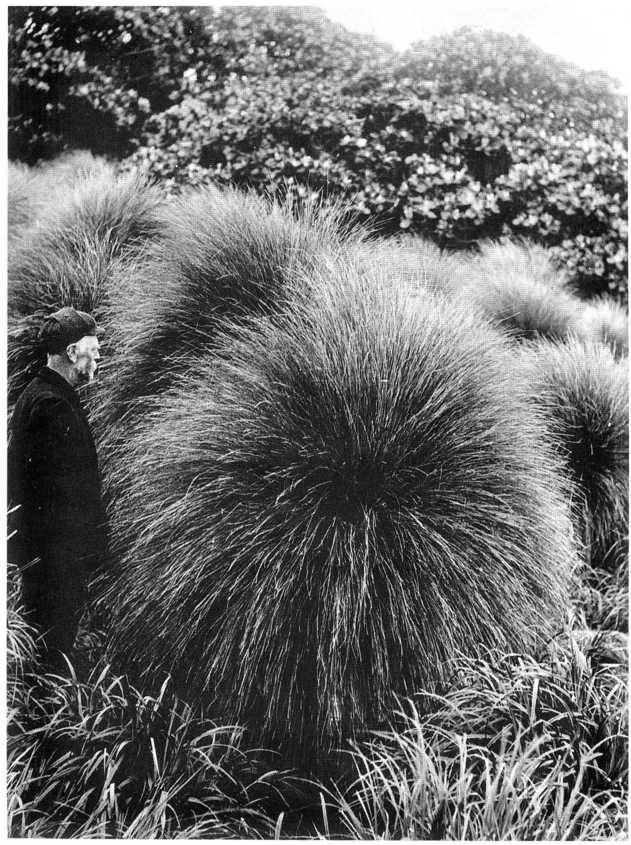
\includegraphics[width=0.5\textwidth]{graphics/figure115cockayne.jpg}
	\centering
	\caption[Leonard Cockayne and a large tussock]{Leonard Cockayne and a large tussock of \BotanicRef{Poa litorosa}[Poa][litorosa] on the Auckland Islands.
	Photo: S. Page.}%
	\label{fig:115cockayne}
\end{SCfigure}
\BotanicRef{Stilbocarpa polaris}[Stilbocarpa][polaris], which belongs to a distinctive genus restricted to the southern extremity of New Zealand and its subantarctic islands, is associated with the tussocks particularly in places enriched by animals.
Although \BotanicRef{Stilbocarpa} belongs to the mostly woody Araliaceae (including \BotanicRef{Pseudopanax}) it is completely herbaceous with large sort leaves, after the style of rhubarb, with blades sometimes as much as half a metre across.
The flower heads are also large with masses of small, yellowish green flowers.
The upper cliff slopes are mostly occupied by a short tussock grassland in which \BotanicRef{Pleurophyllum hookeri}[Pleurophyllum][hookeri] may be a conspicuous component.
\BotanicRef{Pleurophyllum} is a genus restricted to the subantarctic islands, but related to both \BotanicRef{Celmisia} and \BotanicRef{Olearia}.
The three species of \BotanicRef{Pleurophyllum} are notable for rosettes up to a metre or more across of broad, longitudinally ribbed leaves, and for their colourful flower heads.
In \BotanicRef{Pleurophyllum hookeri}[Pleurophyllum][hookeri] the flower heads, coloured reddish purple, are relatively small as their `petals' are greatly reduced.

There is a sudden change of vegetation type on the windswept summit plateau; there is much exposed rock debris and the conspicuous plants are of cushion form.
Some of these are mosses of the genus \BotanicRef{Racomitrium}, but the most common cushion plant is \BotanicRef{Azorella selago}[Azorella][selago] of the Umbelliferae (carrot family).
This is the only occurrence of the genus in the New Zealand region, but it and related genera are prominent in the Andes of South America where some species form huge cushions larger than our `vegetable sheep'.
\BotanicRef{Azorella selago}[Azorella][selago] also occurs at the southern tip of South America and on other islands scattered around the Antarctic Ocean.
The \BotanicRef{Azorella} cushions form a distinctive pattern well described by Gillham:\footnote{\cite{gillham1967sub}}

\begin{quote}
	On leeward slopes with downhill winds \BotanicRef{Azorella} plants coalesce laterally to give terraces as much as a mile long, the ribbon development arising from the prevention of both upward and downward growth by the wind.
	As many as 100 terraces, each about 1½ yards high, may run parallel to the contours to form a gigantic staircase.
\end{quote}

The cushions grow directly on rock or glacial till and form little or no peat, suggesting an affinity with the high alpine cushion moorland of the flat-topped Otago mountains.
Dwarfed versions of the \BotanicRef{Pleurophyllum} and \BotanicRef{Stilbocarpa} grow in the cushions as well as, surprisingly, the \IDX{leather-leaf fern} (\BotanicRef{Pyrrosia serpens}[Pyrrosia][serpens]).
The latter is often common as a sun epiphyte on trees in New Zealand and other species of the genus occupy similar habitats in the Asian tropics.

In all there is a modest total of 40 native species of vascular plants on Macquarie.
Two grasses among these, \IDX{tufted hair-grass} (\BotanicRef{Deschampsia penicillata}[Deschampsia][penicillata]) and \IDX{Cook's poa} (\BotanicRef{Poa hamiltonii}[Poa][hamiltonii]),\footnote{\IDX{Macquarie Island saltgrass} (\BotanicRef{Puccinellia macquariensis}[Puccinellia][macquariensis]) was also thought to be endemic, but has recently been discovered on Campbell Island.} are considered to be endemic although related to other subantarctic species, and three others are not found elsewhere in the New Zealand region, but are shared with several other higher latitude islands as well as the southern tip of South America --- \BotanicRef{Azorella selago}[Azorella][selago], already discussed, \BotanicRef{Acaena adscendens}[Acaena][adscendens] and \BotanicRef{Ranunculus biternatus}[Ranunculus][biternatus].\footnote{\cite{wace1960botany}}

About six of the remaining species are shared only with the New Zealand mainland and the rest are scattered around the subantarctic zone including the New Zealand subantarctic islands, and in some cases the New Zealand mainland or both New Zealand and Australia.

The low endemism of the Macquarie flora and the wide distributions of most of the species indicate recent derivation.
\BotanicRef{Nothofagus} logs, determined anatomically as belonging to South American species, have been washed up on Macquarie, but after such a journey it is unlikely that any seeds would have survived in bark crevices.\footnote{Some seeds can float in the sea and arrive unharmed on distant shores. One such was picked up on the coast of Macquarie and when germinated in Australia turned out to be \BotanicRef{Caesalpinia bonduc}[Caesalpinia][bonduc], widespread in tropical coastal habitats. It could not have survived on Macquarie, but at least it got there.}
Fern spores could have arrived by wind and seeds could have travelled internally or externally with either migratory sea birds or land bird stragglers.

\section{Auckland Islands}

The Auckland Islands are currently credited with 187 native vascular plant species,\footnote{\cite{meurk1982supplementary}}\footnote{\cite{johnson1975vascular}} of which perhaps 6 are endemic and a further 22 are found elsewhere only on other subantarctic islands in the New Zealand region.

The relative richness of the Auckland Islands' flora compared with Macquarie reflects partly their lower latitude (\ang{51}S); partly their larger size (the main Auckland Island and the barely separated Adams Island are about \SI{50}{\kilo\metre} long by \SIrange{10}{30}{\kilo\metre} wide); and partly a less severe climate during the last glaciation which probably allowed some of the previous interglacial flora to survive.
The last is also likely to be true of the Campbell and Antipodes Islands.

The Auckland Islands also contrast topographically with Macquarie in having a very indented eastern coastline and, between the glacially steepened valleys, mostly gradual slopes leading up to ridges and distinct peaks, sometimes flat-topped, up to \SI{668}{\metre} in altitude\figureref{\fullref{fig:116auckland-islands}}.

\begin{figure}[!b]
	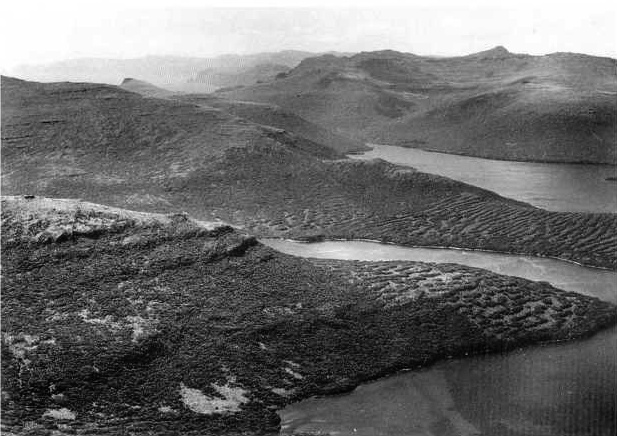
\includegraphics[width=\textwidth]{graphics/figure116auckland-islands.jpg}
	\centering
	\caption[General view of the Auckland Islands from the south]{General view of the Auckland Islands from the south.
	There is a coastal fringe of \IDX{southern rata}[rata!southern] forest (\BotanicRef{Metrosideros umbellata}[Metrosideros][umbellata]) and above that, shrubland with `lanes', then alpine vegetation.
	Photo: P. N. Johnson.}%
	\label{fig:116auckland-islands}
\end{figure}

\subsection{Rata Forest}

The Aucklands are the only islands in the New Zealand subantarctic with forest.
Forest forms a narrow zone up to about \SI{50}{\metre} above sea level on sheltered shorelines and is dominated by \IDX{southern rata}[rata!southern] (\BotanicRef{Metrosideros umbellata}[Metrosideros][umbellata]) in association with \BotanicRef{Dracophyllum longifolium var.\ cockayneanum}[Dracophyllum][longifolium var.\ cockayneanum] and \IDX{haumakoroa} (\BotanicRef{Pseudopanax simplex}[Pseudopanax][simplex]).
Undershrubs are \IDX{stinkwood} (\BotanicRef{Coprosma foetidissima}[Coprosma][foetidissima]), the \BotanicRef{Dracophyllum} and \IDX{weeping matipo} (\BotanicRef{Myrsine divaricata}[Myrsine][divaricata]), while on the forest floor the ferns \IDX{punui} (\BotanicRef{Polystichum vestitum}[Polystichum][vestitum], \IDX{prickly shield fern}), \IDX{southern shore spleenwort} (\BotanicRef{Asplenium scleroprium}[Asplenium][scleroprium]), and \BotanicRef{Blechnum durum}[Blechnum][durum] are abundant in places.
\IDX{Kotukutuku}[kotukutuku] (\BotanicRef{Fuchsia excorticata}[Fuchsia][excorticata]) has been recorded from one locality and the tree fern \IDX{katote} (\BotanicRef{Cyathea smithii}[Cyathea][smithii]) from several sheltered north-facing valley sides in the eastern inlets.
The trees of this forest are unusual in that the lower parts of their trunks and branches are inclined or even prostrate as a result of wind action.
Cockayne\footnote{\cite{cockayne1909ecological}} describes this very graphically:

\begin{quote}
	Everywhere are the massive prostrate and semi-prostrate trunks of the \IDX{southern rata}[rata!southern], sometimes lying close to the ground, at other times forming great arches, or at others again natural bridges over the deep depressions of the forest floor.
\end{quote}

At a few localities at the north-east tip of the main island and on adjacent islets there is also a coastal forest of the large-leaved \IDX{subantarctic tree daisy} (\BotanicRef{Olearia lyallii}[Olearia][lyallii]).
This species has increased its range in Port Ross over the past century and may have reached the Auckland Islands from southern New Zealand as recently as early last century.

\subsection{Shrubland}

Above the narrow forest zone there is a wider belt of `scrub' or shrubland.
Some of the scrub species are also found in the forests, but in the shrubland they are reduced to \SIrange{1}{2}{\metre} in height and when dominated by \IDX{weeping matipo} (\BotanicRef{Myrsine divaricata}[Myrsine][divaricata]) they are so dense as to be almost impenetrable. \IDX{weeping matipo} (\BotanicRef{Myrsine divaricata}[Myrsine][divaricata]) is the dominant species on the upper parts of the valley sides and \IDX{inanga} (\BotanicRef{Dracophyllum longifolium}[Dracophyllum][longifolium]) immediately above the \IDX{rata} forest.
On some gradual slopes the scrub is arranged in an unusual pattern\figureref{\fullref{fig:116auckland-islands}}.
It forms narrow strips, more or less parallel to the contours, which alternate with open lanes with a ground cover of low plants including hard cushions of \IDX{comb sedge} (\BotanicRef{Oreobolus pectinatus}[Oreobolus][pectinatus]), stunted plants of the scrub species, gentians, orchids and scattered tussocks of \IDX{snow tussock}[tussock!snow] (\BotanicRef{Chionochloa antarctica}[Chionochloa][antarctica]).\footnote{\cite{godley1965notes}}
We still await a detailed study which might lead to an explanation of this pattern.

\subsection{Tussock Grassland}

Above \SIrange{300}{400}{\metre} in altitude the shrubland gives way to a grassland dominated by the large yellow-green tussocks of \IDX{snow tussock}[tussock!snow] (\BotanicRef{Chionochloa antarctica}[Chionochloa][antarctica]).
It seems probable that a similar grassland originally occupied the `lanes' within the shrub zone, but these have been greatly modified by the activities of wild pigs.

Several large herbs were a conspicuous feature of the tussock grassland particularly at lower elevations and this is still the case in `Fairchild's Garden' near sea level on Adams Island, where pigs are not present.
Cockayne162 describes the area as `a wonderful collection of stately herbs with immense leaves, and in some cases masses of showy flowers'.

\BotanicRef{Anisotome latifolia}[Anisotome][latifolia] has large, dark green dissected leaves and broad, pink to purple flower heads.
\BotanicRef{Stilbocarpa polaris}[Stilbocarpa][polaris], already described for Macquarie, may also be common.
Two species of \BotanicRef{Pleurophyllum} are conspicuous --- \IDX{great emperor daisy} (\BotanicRef{Pleurophyllum speciosum}[Pleurophyllum][speciosum])\figureref{\fullref{fig:117herbs}} with rosettes of almost circular, pale green longitudinally pleated leaves up to \SI{30}{\centi\metre} in diameter and \BotanicRef{Pleurophyllum criniferum}[Pleurophyllum][criniferum] with even longer, but ascending, leaves up to \SI{1}{\metre} long.
\begin{SCfigure}[1.0][!b]
	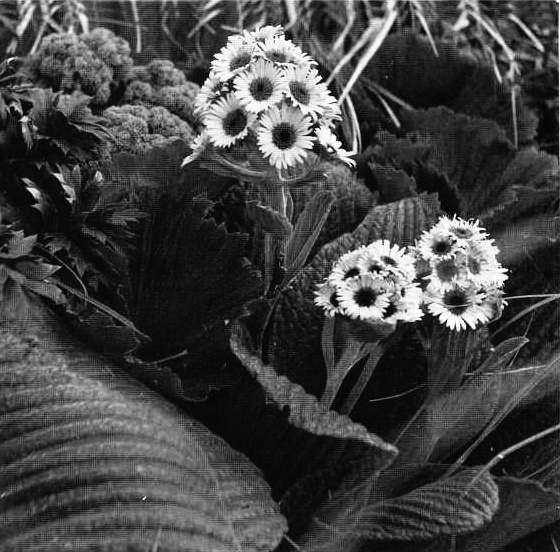
\includegraphics[width=0.66\textwidth]{graphics/figure117herbs.jpg}
	\centering
	\caption[Close up of large herbs on the Auckland Islands]{Close up of large herbs on the Auckland Islands.
	The plants in flower with broad ribbed leaves are \IDX{great emperor daisy} (\BotanicRef{Pleurophyllum speciosum}[Pleurophyllum][speciosum]).
	The dissected leaves on the left are \BotanicRef{Anisotome latifolia}[Anisotome][latifolia] and the rounded leaves with toothed margins centre and right are \BotanicRef{Stilbocarpa polaris}[Stilbocarpa][polaris].
	A flower head of the latter appears in the left background.
	Photo: D. J. Campbell.}%
	\label{fig:117herbs}
\end{SCfigure}
The former has quite large flowers with purple centres and pinkish `petals', while the latter, although its flower heads may be \SI{1.5}{\metre} high, has red, dome-shaped button flowers similar to those of \BotanicRef{Pleurophyllum hookeri}[Pleurophyllum][hookeri].
Towards the upper limits of the garden \IDX{great emperor daisy} (\BotanicRef{Pleurophyllum speciosum}[Pleurophyllum][speciosum]) and \IDX{Ross lily} (\BotanicRef{Bulbinella rossii}[Bulbinella][rossii]) become particularly abundant.
\BotanicRef{Bulbinella rossii}[Bulbinella][rossii] is much larger than its mainland relatives and has broad arching leaves and large orange-yellow flower heads.

\subsection{Bogs}

At higher altitudes, and also in the `lanes' at lower altitudes, on very wet, more or less level sites there is a low plant cover of mat or cushion plants including \BotanicRef{Carpha alpina}[Carpha][alpina], \BotanicRef{Astelia linearis}[Astelia][linearis], \IDX{comb sedge} (\BotanicRef{Oreobolus pectinatus}[Oreobolus][pectinatus]), \BotanicRef{Centrolepis ciliata}[Centrolepis][ciliata] and `glistening green mats' of \BotanicRef{Damnamenia vernicosa}[Damnamenia][vernicosa], an endemic genus formerly included in \BotanicRef{Celmisia}.

\subsection{Fellfield}

Some of the exposed summit peaks have a stony mineral soil with little peat development.
They support a variety of plants, including \BotanicRef{Pleurophyllum hookeri}[Pleurophyllum][hookeri] which is often common, \BotanicRef{Plantago aucklandica}[Plantago][aucklandica] with its large leaf rosettes, \BotanicRef{Ranunculus pinguis}[Ranunculus][pinguis] with unusually large yellow flowers for the size of the plants and \BotanicRef{Myosotis capitata}[Myosotis][capitata] with brilliant dark blue flowers.

\section{Campbell Island}

Campbell Island is found at \SI{51.5}{\degree}S.
Topographically it is similar to the Auckland Islands but is smaller, measuring about \SI{16}{\kilo\metre} by \SI{16}{\kilo\metre}.
It also has fewer vascular species, 128, of which the majority are shared with the Aucklands.\footnote{\cite{oliver1951botanical}}
Four species are considered to be endemic.

It is a little difficult to reconstruct the original vegetation patterns as the island was operated as a sheep station from late last century until 1931 and as a result some palatable species became rare while unpalatable species became more common.
A fence was constructed across the narrow centre of the island in 1970 and all sheep removed from the northern half of the island.
It is encouraging to learn that some species are now recovering strongly north of the fenced.\footnote{\cite{meurk1982regeneration}}

Although not much further south than the Auckland Islands there is no forest fringe on Campbell Island.
Instead up to about \SI{200}{\metre} altitude in sheltered places there is a dense shrubland comprising the endemic \BotanicRef{Dracophyllum scoparium}[Dracophyllum][scoparium] and \IDX{inanga} (\BotanicRef{Dracophyllum longifolium}[Dracophyllum][longifolium]).
Sometimes two species of small-leaved coprosmas and \IDX{weeping matipo} (\BotanicRef{Myrsine divaricata}[Myrsine][divaricata]) can be found mixed with the \BotanicRef{Dracophyllum}, and also scattered through the tussock grassland.

Cockayne162 recognised two zones in the tussock grassland, the lower dominated by \BotanicRef{Poa litorosa}[Poa][litorosa] and the upper by \IDX{snow tussock}[tussock!snow] (\BotanicRef{Chionochloa antarctica}[Chionochloa][antarctica]).
Scattered throughout are several species of herbs and small shrubs, including the two larger species of \BotanicRef{Pleurophyllum}, \IDX{Ross lily} (\BotanicRef{Bulbinella rossii}[Bulbinella][rossii]), \IDX{Campbell Island gentian} (\BotanicRef{Gentiana antarctica}[Gentiana][antarctica]) and the blue-flowered \IDX{Benthams hebe} (\BotanicRef{Hebe benthamii}[Hebe][benthamii]).

The plants of cushion bogs and rocky mountain tops are mostly the same as those of comparable habitats in the Auckland Islands.

\section{Antipodes Island}

At \ang{49}S Antipodes Island is further north than the other vegetated subantarctic islands, but being only \SI{7}{\kilo\metre} by \SI{5}{\kilo\metre} is much the smallest and has a small flora --- about 166 species of which 4 are endemic.\footnote{\cite{williams1982species}}
Above the fringing cliffs the island slopes gradually to a high point of about \SI{400}{\metre}.
The vegetation is almost entirely tussock grassland dominated by \BotanicRef{Poa litorosa}[Poa][litorosa].
Near the shore the tussocks are particularly large and in Cockayne's words they:

\begin{quote}
	grow so closely together out of the wet peaty soil that it is hardly feasible to force a passage between them, and it is much more easy to walk upon their tops, stepping from tussock to tussock.\footnote{\cite{cockayne1909ecological}}
\end{quote}

Further upslope the fern \IDX{punui} (\BotanicRef{Polystichum vestitum}[Polystichum][vestitum]) in its semitree fern form becomes an important component of the grassland, but there is also `much bright-green \BotanicRef{Anisotome antipoda}[Anisotome][antipoda], pale bluish-green \BotanicRef{Acaena antarctica}[Acaena][antarctica] (climbing over the tussocks), and the tender green fern \BotanicRef{Histiopteris incisa}[Histiopteris][incisa]'.
In sheltered places \BotanicRef{Stilbocarpa polaris}[Stilbocarpa][polaris] may form dense stands.
Where ground has been manured by the giant petrel the endemic herb \IDX{Antipodes groundsel} (\BotanicRef{Senecio antipodus}[Senecio][antipodus]) is abundant.

Shrub patches of \BotanicRef{Coprosma antipoda}[Coprosma][antipoda] occur in sheltered gullies.

Localised bogs are largely devoid of tussock grass, but have an abundance of \BotanicRef{Anisotome antipoda}[Anisotome][antipoda], \BotanicRef{Stilbocarpa polaris}[Stilbocarpa][polaris] and patches of \BotanicRef{Coprosma perpusilla}[Coprosma][perpusilla] and the \IDX{much-divided filmy fern} (\BotanicRef{Hymenophyllum multifidum}[Hymenophyllum][multifidum]).

\section{General Comment on the New Zealand Subantarctic Flora}

From this review of the plants of New Zealand's subantarctic islands it is clear that their floras are quite closely related.
In total about 200 species are currently recognised.
In an earlier review Cheeseman\footnote{\cite{cheeseman1909systematic}} estimated that 27.5 per cent of the total New Zealand subantarctic flora was endemic, 69 per cent shared with New Zealand and in some cases other lands, and 3.5 per cent with other circumpolar islands and/or southern South America, but not New Zealand.

The New Zealand mainland and subantarctic island floras are closely related, but the significant level of endemism of the latter suggests that it has had a relatively long history.

\section{Chatham Islands}

These islands lie about \SI{820}{\kilo\metre} east of Banks Peninsula at \ang{44}S.
The main island is about \SI{45}{\kilo\metre} north to south with a narrow waist \SI{8}{\kilo\metre} across, widening to about \SI{50}{\kilo\metre} in the north and to about \SI{25}{\kilo\metre} in the south.
The island is generally low lying with the highest point in the south only \SI{284}{\metre}.
About one quarter of the island's area is taken up by the Te Whanga lagoon and there are a number of other smaller lakes.
Pitt Island, \SI{16}{\kilo\metre} by \SI{8}{\kilo\metre}, a little to the south, is the only other island of any size.

The Chatham Islands are a little greater in area than the Aucklands and lie in milder latitudes, so they have a larger vascular flora of about 320 species with a higher proportion of woody plants.
At least 29 of the species and 8 susbspecific taxa are endemic and the great majority of the remainder are shared with New Zealand.

Rainfall on the main island is moderate, ranging from a minimum of \SI{600}{\milli\metre} in the lowlands to probably over \SI{1200}{\milli\metre} on the southern table land.
Cool south-west winds predominate, atmospheric humidity is high, skies are often cloudy and temperatures are relatively cool for the latitude.
Frosts, however, are rare and a few droughts exceeding 15 days can be expected each year.
It is not a climate that one would expect to lead to the extensive development of peat, but in fact 60 per cent of the land surface is covered by peat and peat soils.
Most of the peat is in raised bogs maintained by rainwater and hence is of low fertility.
Wright,\footnote{\cite{wright1959soils}} who surveyed the soils of Chatham Island, suggests that a high level of salt deposition from strong winds may inhibit decay of plant litter and so encourage peat formation on the many flat or gently sloping sites.

Again there are some difficulties in reconstructing the original vegetation as a long period of Maori occupation was followed by European settlers with their attendant sheep and cattle.
Early botanical accounts, especially that of Cockayne\footnote{\cite{cockayne1902chatham}} early this century, are helpful in determining the nature of the original vegetation cover.
At these earlier times, although there were still extensive forests, a number of the hillslopes and ridges at lower elevations and some ridges at higher elevations were occupied by a low plant cover dominated by bracken fern.
As on the mainland this community was probably induced by Maori fire.

Recently Kelly\footnote{\cite{kelly1983distribution}} and Given and Williams\footnote{\cite{given1984conservation}} have surveyed the remaining areas of native vegetation of the Chathams and the following is largely based on their accounts.

\subsection{Broadleaf Forests}

The forests of the Chatham Islands are relatively low as none of the taller trees of the New Zealand mainland are present.
There are no conifers at all, no beeches (\BotanicRef{Nothofagus}), nor any of the other canopy dominants such as \IDX{tawa} (\BotanicRef{Beilschmiedia tawa}[Beilschmiedia][tawa]), \IDX{kamahi} (\BotanicRef{Weinmannia racemosa}[Weinmannia][racemosa]), \IDX{hinau} (\BotanicRef{Elaeocarpus dentatus}[Elaeocarpus][dentatus]), or northern\index{rata!northern} or \IDX{southern rata}[rata!southern] (\BotanicRef{Metrosideros robusta}[Metrosideros][robusta], \BotanicRef{Metrosideros umbellata}[Metrosideros][umbellata]).
In more open sites a notable absentee is the \IDX{ti kouka} (\BotanicRef{Cordyline australis}[Cordyline][australis], \IDX{cabbage tree}).

On steeper slopes, too well drained to permit the development of peat, the forest is relatively rich in species.
A close canopy at \SIrange{6}{13}{\metre} is dominated by endemic species: \IDX{Chatham Island karamu} (\BotanicRef{Coprosma chathamica}[Coprosma][chathamica]) (the largest species of the genus), \IDX{hoho} (\BotanicRef{Pseudopanax chathamicus}[Pseudopanax][chathamicus]), \IDX{hakina} (\BotanicRef{Melicytus chathamicus}[Melicytus][chathamicus]), \IDX{Chatham Island matipo} (\BotanicRef{Myrsine chathamica}[Myrsine][chathamica]), the striking yellow-flowered \IDX{rautini} (\BotanicRef{Brachyglottis huntii}[Brachyglottis][huntii]), and on more fertile soil the \IDX{nikau palm}, \BotanicRef{Rhopalostylis sapida}[Rhopalostylis][sapida].

Among the few understory species are \IDX{kawakawa} (\BotanicRef{Macropiper excelsum}[Macropiper][excelsum]) and tree ferns, particularly \IDX{rough tree fern} (\BotanicRef{Dicksonia squarrosa}[Dicksonia][squarrosa]) and \IDX{wheki-ponga} (\BotanicRef{Dicksonia fibrosa}[Dicksonia][fibrosa]).
The common vines are \IDX{kareao} (\BotanicRef{Ripogonum scandens}[Ripogonum][scandens], \IDX{supplejack}) and \IDX{pohuehue} (\BotanicRef{Muehlenbeckia australis}[Muehlenbeckia][australis]).
A number of epiphytes are present including the fern \IDX{leather-leaf fern} (\BotanicRef{Pyrrosia serpens}[Pyrrosia][serpens]) and the orchids \IDX{peka-a-waka} (\BotanicRef{Earina mucronata}[Earina][mucronata]) and \IDX{raupeka} (\BotanicRef{Earina autumnalis}[Earina][autumnalis]), but there are no asteliad nests.\footnote{There is, however, a large endemic ground \BotanicRef{Astelia}, \IDX{kakaha} (\BotanicRef{Astelia chathamica}[Astelia][chathamica]), which grows in moist sites in the south of the main island.}
This type of forest is now restricted to gullies in the south of the main island\figureref{\fullref{fig:118chatham-island}} and the southern part of Pitt Island.

\begin{figure}[!b]
	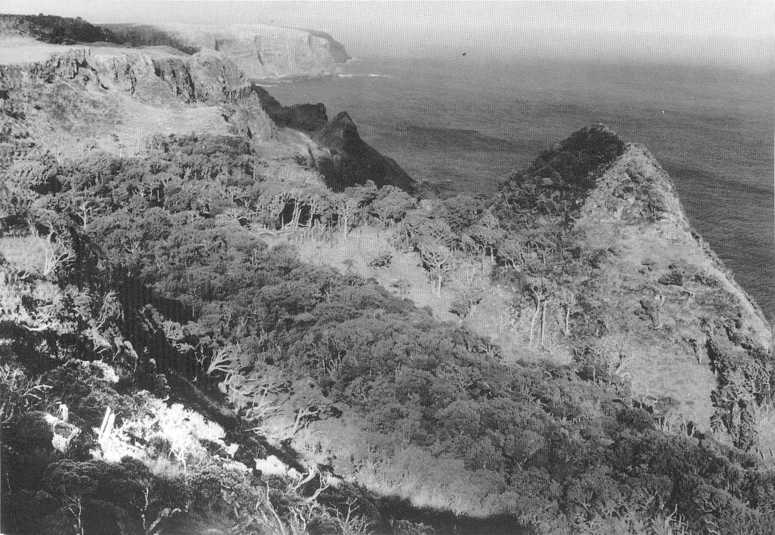
\includegraphics[width=\textwidth]{graphics/figure118chatham-island.jpg}
	\centering
	\caption[Chatham Island, southern cliffs]{Chatham Island.
	Southern cliffs with low forest.
	Photo: D. R. Given.}%
	\label{fig:118chatham-island}
\end{figure}

On more or less level sites in the lowlands, \IDX{karaka} (\BotanicRef{Corynocarpus laevigatus}[Corynocarpus][laevigatus]) dominated where drainage was good, giving way to \IDX{Chatham Island ribbonwood} (\BotanicRef{Plagianthus regius var.\ chathamicus}[Plagianthus][regius var.\ chathamicus]) on the most fertile soils and to \IDX{small-leaved kowhai} (\BotanicRef{Sophora microphylla}[Sophora][microphylla]) on calcareous sediments.
On coastal cliffs and some dune country \IDX{hakapiri} (\BotanicRef{Olearia traversii}[Olearia][traversii]) played a similar role to that of \IDX{pohutukawa} (\BotanicRef{Metrosideros excelsa}[Metrosideros][excelsa]) in the northern North Island.
In swampy situations there was a distinctive forest of this species in combination with \IDX{Chatham Island karamu} (\BotanicRef{Coprosma chathamica}[Coprosma][chathamica]).
These forest types have been almost entirely cleared for farming.

Plant communities associated with bogs\figureref{\fullref{fig:119chatham-island-bog}} are restricted to the main island and these are mostly found on gentle slopes at higher elevations where rainfall is high and mists frequent.

\begin{SCfigure}[1.0][t]
	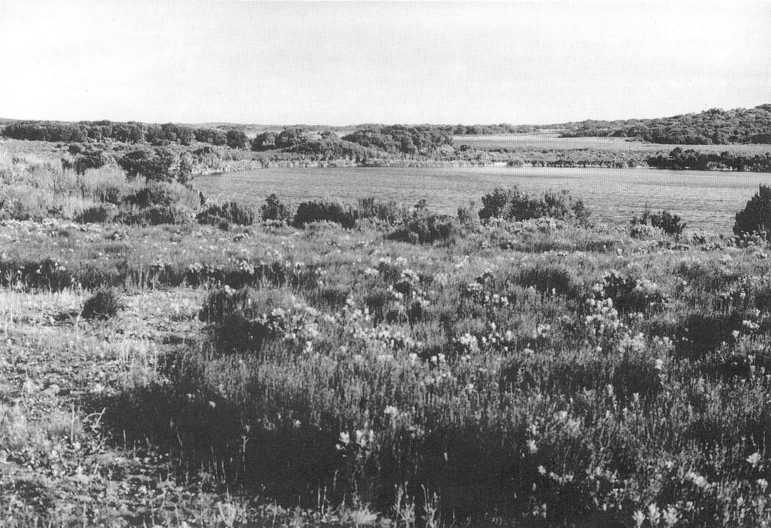
\includegraphics[width=0.66\textwidth]{graphics/figure119chatham-island-bog.jpg}
	\centering
	\caption[Chatham Island bog scene]{Chatham Island.
	Bog scene on the southern tableland.
	Photo: D. R. Given.}%
	\label{fig:119chatham-island-bog}
\end{SCfigure}

\subsection{Bog Forest}

Bog Forest is dominated by \IDX{tarahinau} (\BotanicRef{Dracophyllum arboreum}[Dracophyllum][arboreum], \IDX{Chatham Island grass tree}) and was once very extensive.
It is now largely restricted to the southern tableland.
The \BotanicRef{Dracophyllum} has quite broad leaves when young, but the adult leaves are needle-like.
This species often begins life as an epiphyte on a tree fern and eventually becomes free standing on its own coalesced roots.
Of \IDX{tarahinau} (\BotanicRef{Dracophyllum arboreum}[Dracophyllum][arboreum]) Wright\footnote{\cite{wright1959soils}} says:

\begin{quote}
	In many respects a parallel can be drawn between the \IDX{kauri} tree (\BotanicRef{Agathis australis}[Agathis][australis]) of Northland … and \BotanicRef{Dracophyllum arboreum}[Dracophyllum][arboreum] in the Chathams.
	Both trees accumulate a large mound of organic residues, both condition strongly the soil leaching processes and bring about podsolisation, and both become the dominant species when the soils are sufficiently conditioned.
	The litter in the case of each species consists of leaf, twig and bark residues of high resinous composition.
\end{quote}

The tree ferns \IDX{wheki} (\BotanicRef{Dicksonia squarrosa}[Dicksonia][squarrosa]) and \IDX{wheki-ponga} (\BotanicRef{Dicksonia fibrosa}[Dicksonia][fibrosa]) are prominent in the understory and filmy ferns on the forest floor and, as epiphytes, are a prominent feature.

\subsection{Shrub-Rushland}

In wetter places areas of this type of vegetation formed a mosaic with bog forest and were known as `clears' by the settlers.
The dominant species is the \IDX{Chatham Island bamboo rush}, \BotanicRef{Sporadanthus traversii}[Sporadanthus][traversii], which forms a deep and fibrous peat.
This genus with its single species is restricted to New Zealand and despite the inroads of farming is still to be found locally in the Waikato Basin of the North Island as well as the Chathams.

In the wettest hollows of the bogs Sphagnum moss predominates and shrubs of \IDX{tarahinau} (\BotanicRef{Dracophyllum scoparium}[Dracophyllum][scoparium]) and the purple-flowered \IDX{hanga-tare} (\BotanicRef{Olearia semidentata}[Olearia][semidentata], \IDX{Chatham Island aster}) are scattered throughout.
Most of the `clears' have been completely altered by repeated burning.

A low shrubbery dominated by the endemic \IDX{pouteretere} (\BotanicRef{Styphelia robusta}[Styphelia][robusta]) occupies dry ridges in the peatlands of the southern tableland.

\subsection{Coastal Communities}

A full range of coastal habitats, from sand dunes to rocky cliffs, can be found in the Chatham Islands.
A number of the species are the familiar plants of such sites on the New Zealand mainland, but there are also some notable endemics.
Among these, certain large herbs once formed a band of lush vegetation at the top of many sandy and stony storm beaches: the nettle \IDX{onga} (\BotanicRef{Urtica australis}[Urtica][australis]), \IDX{Chatham Island sow thistle} (\BotanicRef{Embergeria grandifolius}[Embergeria][grandifolius]) and \IDX{kopakopa} (\BotanicRef{Myosotidium hortensia}[Myosotidium][hortensia]).
\BotanicRef{Myosotidium hortensia}[Myosotidium][hortensia], now widely cultivated, could be called a giant forget-me-not.
The leaves, like those of \BotanicRef{Stilbocarpa} in the subantarctic, are rhubarb-like and almost fleshy and the flowers in large heads are blue in the centre grading outwards to white.
It is a plant stock find very palatable and is now quite rare.
Today's sand dunes are dominated by the introduced marram grass.

Endemics of sea cliffs include \IDX{Chatham Island koromiko} (\BotanicRef{Hebe chathamica}[Hebe][chathamica]), \IDX{Dieffenback's koromiko} (\BotanicRef{Hebe dieffenbachii}[Hebe][dieffenbachii]) and the grasses \IDX{Chatham Islands poa} (\BotanicRef{Poa chathamica}[Poa][chathamica]) and \IDX{Cox's fescue} (\BotanicRef{Festuca coxii}[Festuca][coxii]).
\IDX{Kopakopa}[kopakopa] (\BotanicRef{Myosotidium hortensia}[Myosotidium][hortensia]) may still be found in inaccessible places.
Dense shrubberies of \BotanicRef{Olearia chathamica}[Olearia][chathamica] may be prominent along cliff tops.
A large, grey-green, remarkably soft-leaved \BotanicRef{Aciphylla}, \IDX{Dieffenbach’s speargrass} (\BotanicRef{Aciphylla dieffenbachii}[Aciphylla][dieffenbachii]), was formerly common along the southern cliffs of the main island and is still frequent on Pitt Island.
A smaller species, \IDX{taramea karupuru} (\BotanicRef{Aciphylla traversii}[Aciphylla][traversii], \IDX{Chatham Island speargrass}), is a plant of tableland bogs, but it, too, has been reduced by stock.

In highly fertile peaty places riddled with muttonbird burrows, grow luxuriant masses of \IDX{tataki} (\BotanicRef{Carex trifida}[Carex][trifida]) and the endemics \IDX{Chatham Island button daisy} (\BotanicRef{Leptinella featherstonii}[Leptinella][featherstonii]) and \BotanicRef{Senecio radiolatus}[Senecio][radiolatus].
Such sites are now confined to the smaller islands.

With their absence of groups of poor dispersal ability, particularly conifers, the Chathams have an isolated oceanic rather than a continental flora.
New Zealand seems to be the principal source area but, as with the subantarctic islands, the presence of a significant element of distinctive endemics indicates quite a long period in isolation.

\section{Subtropical Islands}

\section{Kermadec Islands}

The Kermadecs are a row of small islands about \SI{1000}{\kilo\metre} north-east of New Zealand.
The largest and northernmost island is Raoul at \ang{29}S, but it measures only about \SI{10}{\kilo\metre} by \SI{8}{\kilo\metre} with a highest point of 520 m.
It is a volcano which is active from time to time.
Macauley Island, the next island to the south, is only \SI{2}{\kilo\metre} long, and the southernmost island with a significant flora, Curtis, is even smaller.

With the warm, humid climate, forest is the predominant vegetation cover.\footnote{\cite{sykes1977annotated}}
On Raoul Island Oliver\footnote{\cite{oliver1910vegetation}} distinguished a lower altitude `dry' forest and above \SIrange{200}{300}{\metre} a higher altitude `wet' forest.
\IDX{Kermadec pohutukawa} (\BotanicRef{Metrosideros kermadecensis}[Metrosideros][kermadecensis]), up to \SI{20}{\metre} tall, dominates the canopy of the lower forest.
\IDX{Karaka}[karaka]s (\BotanicRef{Corynocarpus laevigatus}[Corynocarpus][laevigatus]) and \IDX{ngaio}s (\BotanicRef{Myoporum obscurum}[Myoporum][obscurum], closely related to \BotanicRef{Myoporum laetum}[Myoporum][laetum]) also reach \SI{20}{\metre} in height in sheltered places; considerably greater dimensions than they usually attain in New Zealand.
There is a rather sparse subcanopy dominated by \IDX{Kermadec mapou} (\BotanicRef{Myrsine kermadecensis}[Myrsine][kermadecensis]) but also with \IDX{mahoe} (\BotanicRef{Melicytus ramiflorus}[Melicytus][ramiflorus]), \IDX{ngaio}, \IDX{karaka}, \IDX{wharangi} (\BotanicRef{Melicope ternata}[Melicope][ternata]), \BotanicRef{Coprosma acutifolia}[Coprosma][acutifolia], the nikau palm relative \IDX{Kermadec nikau} (\BotanicRef{Rhopalostylis baueri var.\ cheesemanii}[Rhopalostylis][baueri var.\ cheesemanii]) (sometimes forming picturesque groves), \IDX{Milnes tree fern} (\BotanicRef{Cyathea milnei}[Cyathea][milnei]), and the endemic \IDX{Kermadec poplar} (\BotanicRef{Homalanthus polyandrus}[Homalanthus][polyandrus]), now increasing markedly owing to the great reduction in numbers of goats.
The fern \BotanicRef{Pteris comans}[Pteris][comans], up to \SI{2}{\metre} high, is the commonest plant of the forest floor (although in many places the introduced aroid \BotanicRef{Alocasia macrorhiza}[Alocasia][macrorhiza] is dominant), but there are also a number of other ferns and the large leaved form of \IDX{kawakawa} (\BotanicRef{Macropiper excelsum f.\ psittacorum}[Macropiper][excelsum f.\ psittacorum]) along the north side.

The upper or `wet' forest is mostly about \SI{10}{\metre} high and comprises the same species as the lower forest with the addition of \IDX{Kermadec Islands hutu} (\BotanicRef{Ascarina lucida var.\ lanceolata}[Ascarina][lucida var.\ lanceolata]), which dominates the understorey, and, in a few places, the \IDX{Kermadec tree fern} (\BotanicRef{Cyathea kermadecensis}[Cyathea][kermadecensis]).
\BotanicRef{Cyathea kermadecensis}[Cyathea][kermadecensis] occasionally forms impressive groves where some specimens, according to Oliver, have trunk bases \SIrange{1}{2}{\metre} in diameter.
The forest floor and trunks and branches of trees are covered with mosses and ferns.
Common epiphytes familiar to New Zealanders are the ferns \BotanicRef{Thymatosorus diversifolius}[Thymatosorus][diversifolius], \IDX{leather-leaf fern} (\BotanicRef{Pyrrosia serpens}[Pyrrosia][serpens]), \IDX{drooping spleenwort} (\BotanicRef{Asplenium flaccidum}[Asplenium][flaccidum]) and \IDX{irirangi} (\BotanicRef{Hymenophyllum demissum}[Hymenophyllum][demissum]).
Much rarer are \IDX{clubmoss} (\BotanicRef{Lycopodium varium}[Lycopodium][varium]), \IDX{fork fern} (\BotanicRef{Tmesipteris lanceolata}[Tmesipteris][lanceolata]) and \IDX{veined bristle fern} (\BotanicRef{Trichomanes venosum}[Trichomanes][venosum]).
There are no lianes in the Kermadec forests and no large epiphytes apart from the occasional \IDX{
Kermadec five finger} (\BotanicRef{Pseudopanax arboreus var.\ kermadecensis}[Pseudopanax][arboreus var.\ kermadecensis]) and \IDX{Kermadec pohutukawa} (\BotanicRef{Metrosideros kermadecensis}[Metrosideros][kermadecensis]).
The only other flowering plant epiphyte is \BotanicRef{Peperomia urvilleana}[Peperomia][urvilleana].

Close to the sea in many places, as in New Zealand, is a dense shrubbery of the \IDX{ngaio} relative \BotanicRef{Myoporum obscurum}[Myoporum][obscurum].
Probably \IDX{ngaio} shrubbery was the dominant vegetation on Macauley Island, but the fires of early whalers and the activities of goats have almost eliminated the woody vegetation of that island.

In open, mostly rocky coastal habitats are a number of herbaceous plants, including a few ferns.
Most of these grow in similar sites in New Zealand.
\IDX{Taupata}[taupata] (\BotanicRef{Coprosma petiolata}[Coprosma][petiolata]) is a common endemic coastal shrub.

The total vascular flora of the Kermadecs is 113 species.
Eighteen species and three varieties are considered to be endemic and those with New Zealand affinities are \IDX{taupata} (\BotanicRef{Coprosma petiolata}[Coprosma][petiolata]) and \BotanicRef{Coprosma acutifolia}[Coprosma][acutifolia], the tree ferns \IDX{Milnes tree fern} (\BotanicRef{Cyathea milnei}[Cyathea][milnei]) and \IDX{Kermadec tree fern} (\BotanicRef{Cyathea kermadecensis}[Cyathea][kermadecensis]), \IDX{Kermadec five-finger} (\BotanicRef{Pseudopanax arboreus var.\ kermadecensis}[Pseudopanax][arboreus var.\ kermadecensis]) (close to the New Zealand variety and like it sometimes a tree fern epiphyte), \BotanicRef{Metrosideros kermadecensis}[Metrosideros][kermadecensis], (known as the \IDX{Kermadec pohutukawa} in cultivation in New Zealand; it has shorter, more rounded leaves than \IDX{pohutukawa} (\BotanicRef{Metrosideros excelsa}[Metrosideros][excelsa])), \BotanicRef{Myoporum obscurum}[Myoporum][obscurum], \IDX{Kermadec koromiko} (\BotanicRef{Hebe breviracemosa}[Hebe][breviracemosa]) (now probably extinct) and the palm \IDX{Kermadec nikau} (\BotanicRef{Rhopalostylis baueri var.\ cheesemanii}[Rhopalostylis][baueri var.\ cheesemanii]).

About 80 of the 113 Kermadec species are shared with New Zealand, but as many of them are also to be found elsewhere in the Pacific and in eastern Australia, they have not necessarily all been derived from New Zealand.

The Kermadec Islands have arisen as volcanoes in isolation and it seems likely that their flora has resulted from long distance dispersal, with New Zealand probably the most important source.

\section[Norfolk Island]{Norfolk Island\thinspace\footnote{\cite{laing1915revised}}\footnote{\cite{turner1968conservation}}\footnote{\cite{green1970notes}}\footnote{\cite{green1979observations}}}

At the same latitude as Raoul Island, but \SI{1400}{\kilo\metre} to the west, Norfolk Island is equally small with the even smaller Phillip Island a little to the south.
The two islands are remnants of a long extinct volcano.
Norfolk is fringed by cliffs and has a plateau-like surface rising gradually to a high point only \SI{350}{\metre} above sea level.
Little of the original vegetation remains as it was largely removed early last century as a result of a penal settlement being established and the subsequent settling of the island by the descendants of the `Bounty' mutineers from Pitcairn in 1856.
It has been prevented from re-establishing since that time by fires and grazing of stock.
The climate, although a little drier than the Kermadecs, is suitable for forest and records of early explorers show that the island was originally covered with dense forest.
The most notable species of the flora is the so-called \IDX{Norfolk Island pine} (\BotanicRef{Araucaria heterophylla}[Araucaria][heterophylla]), the only conifer native to any of the outlying islands.
This has survived rather better than some of the other species and is still a distinctive feature of the landscape.
In the original forest the Araucarias would have been emergent above the main canopy and may also have formed pure groves on less fertile sites as is the case with some of the Araucarias in \IDX{New Caledonia}.

The lower strata of the forest included species related to or the same as New Zealand species: \BotanicRef{Nestegis apetala}[Nestegis][apetala], the palm \BotanicRef{Rhopalostylis baueri var.\ baueri}[Rhopalostylis][baueri var.\ baueri], the tree fern \BotanicRef{Cyathea robusta}[Cyathea][robusta], \IDX{mahoe} (\BotanicRef{Melicytus ramiflorus}[Melicytus][ramiflorus]), \IDX{kawakawa} (\BotanicRef{Macropiper excelsum f.\ psittacorum}[Macropiper][excelsum f.\ psittacorum]), \BotanicRef{Myoporum obscurum}[Myoporum][obscurum], \IDX{Three Kings cabbage tree} (\BotanicRef{Cordyline obtecta}[Cordyline][obtecta]), \BotanicRef{Pennantia endlicheri}[Pennantia][endlicheri] and species of \BotanicRef{Meryta}.
Unlike the Kermadecs, Norfolk Island has locally abundant lianes which include \IDX{kiekie} (\BotanicRef{Freycinetia baueri var.\ baueri}[Freycinetia][baueri var.\ baueri]) and \IDX{pohuehue} (\BotanicRef{Muehlenbeckia australis}[Muehlenbeckia][australis]), shared with New Zealand, and species of \BotanicRef{Clematis}, \BotanicRef{Passiflora}, \BotanicRef{Ripogonum} and several other genera.
Vascular epiphytes also are more numerous --- species of the orchid genera \BotanicRef{Dendrobium} and \BotanicRef{Bulbophyllum}, and species of \BotanicRef{Peperomia} and among ferns \BotanicRef{Asplenium australasicum}[Asplenium][australasicum], \IDX{sickle spleenwort} (\BotanicRef{Asplenium polyodon}[Asplenium][polyodon]), \BotanicRef{Pyrrosia confluens}[Pyrrosia][confluens] and the fern ally \IDX{fork fern} (\BotanicRef{Tmesipteris forsteri}[Tmesipteris][forsteri]).

The cliffs are occupied mostly by species widespread in the south-west Pacific, with the exception of \IDX{harakeke} (\BotanicRef{Phormium tenax}[Phormium][tenax]), shared with New Zealand, and \IDX{taupata} (\BotanicRef{Coprosma baueri}[Coprosma][baueri]), which occupies similar sites to its very close relatives \BotanicRef{Coprosma repens}[Coprosma][repens] in New Zealand and \BotanicRef{Coprosma petiolata}[Coprosma][petiolata] in the Kermadecs.

With about 174 species Norfolk has a rather larger flora than the Kermadecs.
Of these perhaps 50 are endemic.

About 76 species are shared with New Zealand and, often, elsewhere.

\section[Lord Howe Island]{Lord Howe Island\thinspace\footnote{\cite{oliver1896vegetation}}\footnote{\cite{green1979observations}}\footnote{\cite{hutton1986lord}}}

Lying about \SI{850}{\kilo\metre} west of Norfolk at \ang{31}S Lord Howe Island is much closer to Australia (\SI{600}{\kilo\metre}) than New Zealand (\SI{1300}{\kilo\metre}).
The island is crescent shaped and about \SI{10}{\kilo\metre} long by \SI{3}{\kilo\metre} at its widest.
Like Norfolk it is the remnant of a long extinct volcano, but it is much more mountainous and has much of its original vegetation largely intact.
The northern half of the island includes groups of hills, but in the south are two steep mountains --- Mt.
Gower (875 m) and Mt.
Lidgbird (763 m)\figureref{\fullref{fig:120lord-howe-island}}.
Mild to warm temperatures and ample rainfall support dense forest over most of the island, with shrub associations near the sea on cliffs, and on the mountain tops.

\begin{SCfigure}[1.0][t]
	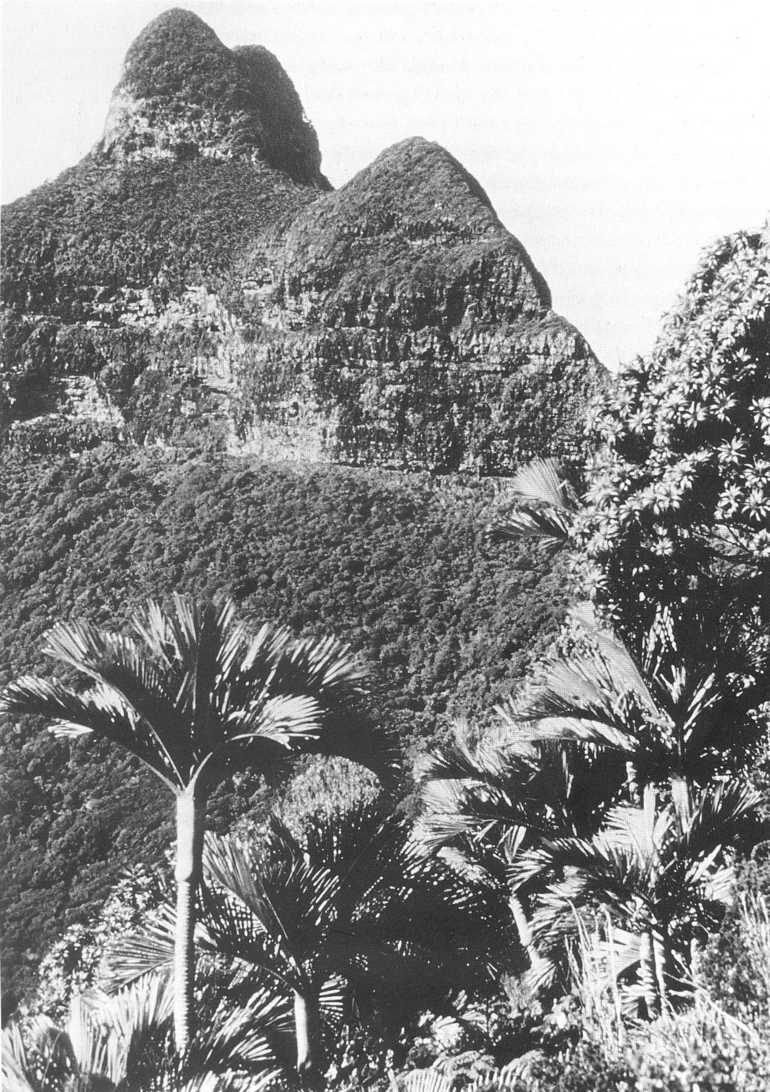
\includegraphics[width=0.66\textwidth]{graphics/figure120lord-howe-island.jpg}
	\centering
	\caption[Lord Howe Island]{Lord Howe Island.
	Mt. Lidgbird with \BotanicRef{Howea} palms in the foreground.
	Photo: G. W. Gibbs.}%
	\label{fig:120lord-howe-island}
\end{SCfigure}

Up to about \SI{300}{\metre} there is a relatively tall forest with scattered emergent trees to \SI{20}{\metre} in height.
In some places and particularly at lower elevations the emergents are of the endemic \BotanicRef{Ficus columnaris}[Ficus][columnaris], one of the species of the fig genus known as banyans.
In these the spreading branches are supported by innumerable trunk-like `column roots'.
Elsewhere and tending to be at higher elevations the emergents are \BotanicRef{Cleistocalyx fullageri}[Cleistocalyx][fullageri], which belongs to the fleshy-fruited subfamily of the family Myrtaceae.
The main canopy of the lowland forest is about \SI{15}{\metre} high and composed of a mixture of species of genera not found in New Zealand.
Conspicuous are some of the handsome \IDX{Kentia palm}s for which Lord Howe is noted --- \BotanicRef{Howea forsteriana}[Howea][forsteriana] and \BotanicRef{Howea belmoreana}[Howea][belmoreana] at lower elevations with \BotanicRef{Hedescepe canterburyana}[Hedescepe][canterburyana] higher up.
Both genera are endemic.
Among the subcanopy trees and shrubs New Zealand relatives are more frequent --- \BotanicRef{Coprosma putida}[Coprosma][putida], \BotanicRef{Geniostoma petiolosum}[Geniostoma][petiolosum], \IDX{Lord Howe kowhai} (\BotanicRef{Sophora howinsula}[Sophora][howinsula]), \BotanicRef{Myrsine platystigma}[Myrsine][platystigma], \IDX{Tasmanian ngaio} (\BotanicRef{Myoporum insulare}[Myoporum][insulare]), \BotanicRef{Dysoxylum pachyphyllum}[Dysoxylum][pachyphyllum], \IDX{kawakawa} (\BotanicRef{Macropiper excelsum}[Macropiper][excelsum]) and \BotanicRef{Bubbia howeana}[Bubbia][howeana].
\BotanicRef{Bubbia} belongs to a primitive flowering family, Winteraceae, which also includes the New Zealand \BotanicRef{Pseudowintera}.
Ferns, sedges and grasses are common on the forest floor.
Lianes are abundant, but, except for a \BotanicRef{Clematis}, belong to genera not represented in New Zealand.
Epiphytes are infrequent.

Above \SI{300}{\metre} altitude there is a change to a montane low forest without emergents.
A number of the lower altitude species are present here with the addition of \BotanicRef{Dracophyllum fitzgeraldii}[Dracophyllum][fitzgeraldii], \BotanicRef{Metrosideros nervulosa}[Metrosideros][nervulosa] and \BotanicRef{Olearia ballii}[Olearia][ballii].
The Howea palms are replaced by \BotanicRef{Hedyscepe canterburyana}[Hedyscepe][canterburyana].
Lianes and epiphytes are uncommon in this forest.

On the mountain summits is a low forest or shrubbery \SIrange{3}{4}{\metre} high in which tree ferns, \BotanicRef{Dracophyllum fitzgeraldii}[Dracophyllum][fitzgeraldii] and the palms \BotanicRef{Hedyscepe canterburyana}[Hedyscepe][canterburyana] and \BotanicRef{Lepidorrhachis mooreana}[Lepidorrhachis][mooreana] are conspicuous.
Other species from lower altitudes are also present.
Higher altitude species are \BotanicRef{Negria rhabdothamnoides}[Negria][rhabdothamnoides] (an endemic genus related to \BotanicRef{Rhabdothamnus} of New Zealand), \BotanicRef{Corokia carpodetoides}[Corokia][carpodetoides], \BotanicRef{Coprosma lanceolaris}[Coprosma][lanceolaris], and in more open places \BotanicRef{Leptospermum flavescens}[Leptospermum][flavescens] and \IDX{mapere} (\BotanicRef{Gahnia xanthocarpa}[Gahnia][xanthocarpa]).
Ferns are abundant on the ground, and epiphytic ferns, mosses and lichens on the branches of the trees and shrubs.

At most places along the coast there is a narrow zone of shrubs tolerant of salt spray.
A number of species are present, but only \BotanicRef{Coprosma prisca}[Coprosma][prisca] provides a link with New Zealand.

With about 230 vascular species\footnote{\cite{rodd1983census}} Lord Howe has the richest of the subtropical floras resulting no doubt from its more varied topography and nearness to Australia.
About 75 species or a bit less than one third are considered to be endemic.
Included among them is \BotanicRef{Carmichaelia exsul}[Carmichaelia][exsul], the only member of the genus occurring outside New Zealand.

About 70 species are shared by New Zealand and Lord Howe, but most of these occur in a number of other places as well.

\section{General Comments on the Floras of the Subtropical Islands}

The relatively small total number of species and the few not very distinct endemics indicate that the Kermadecs, like Macquarie, have gained their flora by long distance dispersal in fairly recent geological times.
By contrast the larger floras of Norfolk and Lord Howe with their larger numbers of mostly distinctive endemics, including some endemic genera, suggest a much longer history with the possibility of land connections as well as long distance dispersal being involved.
Both islands stand on submarine ridges of continental crust and there could have been a succession of volcanic islands in their vicinity, allowing floral continuity over a long period of time, perhaps from when the ridges were still emergent.
Thus related species in New Zealand and, say, Lord Howe Island may have resulted from long distance dispersal in either direction at various times followed by divergent evolution, or from two populations of an ancestral form separated following submergence of the Lord Howe Rise.
The suggestion of some sort of long term land continuity at the sites of Lord Howe and Norfolk is supported by the presence on each of these islands of at least one species belonging to groups considered to have poor dispersal ability: on Norfolk the conifer \IDX{Norfolk Island pine} (\BotanicRef{Araucaria heterophylla}[Araucaria][heterophylla]), related to but distinct from \BotanicRef{Araucaria columnaris}[Araucaria][columnaris] of New Caledonia; and on Lord Howe \BotanicRef{Bubbia howeana}[Bubbia][howeana] belonging to the primitive flowering family Winteraceae whose members are also considered to be unlikely to cross wide ocean gaps.

At least some species shared by New Zealand and the subtropical islands have presumably achieved their widely disjunct distributions more recently by long distance dispersal.
